\chapter{量级分析实战：每个小参数都用数字检查}
\label{hall:ordering}
\section{量级分析怎样做，怎样不做}
量级分析不是把一个系数说成“小”就删除。做法是选定目标方程、目标分量、目标区域和变化尺度，将各项除以\emph{同一个参考量}。一旦在某点参考项因对称性等于零，就应换参考量或直接比较剩余项，不能继续用原来的比值。

设磁场变化为$\Delta B\sim B$，电流变化尺度为$\ell_B$，压强变化尺度为$\ell_p$，流速尺度为$U$，时间尺度为$\tau$。注意这里的$\ell_B$可以是电流片半厚度，远小于整个装置长度$L$。用安培定律估计
\begin{equation}
J\sim\frac{B}{\mu_0\ell_B},\qquad
U_d\equiv\frac{J}{en}\sim\frac{B}{\mu_0en\ell_B}.
\end{equation}
这里$U_d$是相对流速，不是碰撞频率。也可以直接从电流定义写成
\begin{equation}
U_d\equiv |\vct u_i-\vct u_e|\sim\frac{B}{\mu_0en\ell_B}.
\end{equation}
\textbf{这一估计要求磁场实际在$\ell_B$内改变了同阶幅度。}强导场$B_g$若基本不变，不能把总磁场$B_g$直接放在$J\sim B/(\mu_0\ell_B)$的分子；应该用实际变化的场分量。

\section{惯性长度、回旋半径与Alfvén时间的关系}
定义
\begin{align}
\omega_{ps}&=\sqrt{\frac{n_sq_s^2}{\epsilon_0m_s}},&d_s&=\frac{c}{\omega_{ps}},\\
\Omega_i&=\frac{eB}{m_i},&|\Omega_e|&=\frac{eB}{m_e},&
V_A&=\frac{B}{\sqrt{\mu_0nm_i}}.
\end{align}
利用$c^2=1/(\mu_0\epsilon_0)$，逐步化简
\begin{align}
d_i&=\sqrt{\frac{m_i}{\mu_0ne^2}},\\
\frac{V_A}{\Omega_i}
&=\frac{B}{\sqrt{\mu_0nm_i}}\frac{m_i}{eB}
=\sqrt{\frac{m_i}{\mu_0ne^2}}=d_i,\\
\frac{d_e}{d_i}&=\sqrt{\frac{m_e}{m_i}}=0.02334.
\end{align}
因此$\ell/V_A$和离子回旋时间$\Omega_i^{-1}$的比值恰为$\ell/d_i$。这解释了为什么Alfvén型运动逐渐逼近$d_i$时，离子不能简单维持原来的磁化流体响应。

惯性长度不是回旋半径。采用$v_{ti}=\sqrt{2\Theta_i/m_i}$，有
\begin{align}
\rho_i&=v_{ti}/\Omega_i,&
\beta_i&=\frac{2\mu_0n\Theta_i}{B^2},\\
\left(\frac{\rho_i}{d_i}\right)^2
&=\frac{2\Theta_i/m_i}{V_A^2}=\beta_i,
&\frac{\rho_i}{d_i}&=\sqrt{\beta_i}.
\end{align}
同理$\rho_e/d_e=\sqrt{\beta_e}$。强导场理论中还常出现离子声回旋半径
\begin{equation}
\rho_s=\frac{\sqrt{\Theta_e/m_i}}{\Omega_i},\qquad
\frac{\rho_s}{d_i}=\sqrt{\frac{\beta_e}{2}}.
\end{equation}
这里声速只取等温电子贡献；若包含离子温度和绝热指数，会出现其他定义。\emph{没有一个$d_i$能替代所有几何与beta下的非MHD尺度。}

\section{把广义欧姆定律逐项无量纲化}
\subsection{Hall项相对理想对流项}
取$E_0=UB$。暂不考虑角度使叉积变小，则
\begin{align}
\frac{E_H}{E_0}&\sim\frac{JB/(en)}{UB}
=\frac{B}{\mu_0en\ell_BU},\\
\frac{B}{\mu_0en}&=V_Ad_i,\\
\boxed{\frac{E_H}{E_0}\sim\frac{V_A}{U}\frac{d_i}{\ell_B}}.
\end{align}
只有取$U\sim V_A$时才能简写成$d_i/\ell_B$。入流速度常小于$V_A$，若比较入流方向对应的理想电场，就必须保留$V_A/U$。同时$\J\parallel\B$时Hall叉积为零，标量上界不是实际该分量的数值。

\subsection{标量电子压强项}
以$|\nabla p_e|\sim p_e/\ell_p$估计，有
\begin{align}
\frac{E_p}{E_0}&\sim\frac{p_e}{en\ell_pUB}
=\frac{\Theta_e}{e\ell_pUB}\\
&=\frac{\beta_e}{2}\frac{V_A}{U}\frac{d_i}{\ell_p}.
\end{align}
这一步只估计压强梯度\emph{电场幅度}。它在感应方程中的重要性还取决于旋度：若$p_e=p_e(n)$，此项为梯度，其旋度为零，可以产生电势却不改变磁场。张量压力的非对角项不受相同结论限制。

\subsection{电阻项}
\begin{equation}
\frac{E_\eta}{E_0}\sim\frac{\eta J}{UB}
=\frac{\eta}{\mu_0U\ell_B}
=\frac{D_\eta}{U\ell_B}
\equiv R_m(\ell_B,U)^{-1}.
\end{equation}
$R_m$为该速度与尺度的磁雷诺数。取$U=V_A,\ell_B=L$时通常称$S_L=LV_A/D_\eta$为Lundquist数。一个系统可以有巨大$S_L$，同时在局地薄层里有不可忽略的电阻项。

\subsection{电子惯性：保留时间与空间两种判断}
一般形式先写
\begin{equation}
\frac{E_{m_e}}{UB}\sim\frac{m_e}{eUB}
\left(\frac{U_e}{\tau}+\frac{U_e^2}{\ell_e}\right).
\end{equation}
若只比较电子惯性与电子洛伦兹项$U_eB$，则时间项的比值为$1/(|\Omega_e|\tau)$，对流项为$U_e/(|\Omega_e|\ell_e)$。它们分别是演化时间和穿越时间能否比回旋时间长的条件。

在电子流主导电流、$U_e\sim U_d=V_Ad_i/\ell$且所有局地梯度尺度同阶时，再与Hall量级$U_dB$比较：
\begin{align}
\frac{(m_e/e)U_e^2/\ell}{U_dB}
&\sim\frac{m_eV_Ad_i}{eB\ell^2}
=\frac{m_e}{m_i}\frac{d_i^2}{\ell^2}
=\boxed{\frac{d_e^2}{\ell^2}}.
\end{align}
这个著名比值并不适用于任意速度和几何。实际重联中电子出流沿$x$变化，电流层沿$y$很薄，两个梯度尺度可能不同，必须回到$\vct u_e\cdot\nabla\vct u_e$逐项算。

\section{准中性、忽略位移电流和无碰撞是三种判断}
电子Debye长度为$\lambda_{De}=\sqrt{\epsilon_0\Theta_e/(ne^2)}$。若电势能幅度$e\phi\sim\Theta_e$且变化尺度为$\ell$，Gauss定律给
\begin{equation}
\frac{|n_i-n_e|}{n}\sim\frac{\epsilon_0\phi}{en\ell^2}
\sim\left(\frac{\lambda_{De}}{\ell}\right)^2.
\end{equation}
若$e\phi/\Theta_e$很大，应再乘这个因子。准中性不是把电场设为零；一个很小的电荷差就能维持有限电场。

位移电流相对传导电流，在$E\sim UB$、$\tau\sim\ell/U$、$J\sim B/(\mu_0\ell)$的低频排序中为
\begin{equation}
\frac{\epsilon_0\partial_tE}{J}
\sim\frac{\epsilon_0 UB}{(\ell/U)}\frac{\mu_0\ell}{B}
=\frac{U^2}{c^2}.
\end{equation}
对高频波若$E/B$不同，这个估计要重做。无碰撞则比较$\nu\tau$和$\lambda_{\rm mfp}/\ell$，与Debye长度不是一回事；几乎完全准中性的磁层等离子体仍可能极为无碰撞。

\section{四组教学输入与全部算得的尺度}
以下四组数字均为\textbf{自设教学参数}，分别代表高密度碰撞等离子体、实验室、磁层和日冕的量级，不对应任何指定放电、事件或模拟。默认全电离氢、真实质量比、弱耦合；高密度低温例还需额外假定中性、辐射和反应可忽略。参数表不是四个完整的自洽平衡解。

碰撞采用常用的Maxwell电子--离子频率估计，$Z=1$：
\begin{align}
\nu_{ei}&=\frac{4\sqrt{2\pi}\,ne^4\ln\Lambda}
{3(4\pi\epsilon_0)^2\sqrt{m_e}\,\Theta_e^{3/2}},\\
&\simeq 2.91\times10^{-6}\frac{n[\mathrm{cm^{-3}}]\ln\Lambda}{T_e[\mathrm{eV}]^{3/2}}\ \mathrm{s^{-1}}.
\end{align}
定义\emph{简单拖曳电阻率}$\eta_D=m_e\nu_{ei}/(ne^2)$，并令$D_\eta=\eta_D/\mu_0$。这并非完整Braginskii输运：电子--电子碰撞对分布的改变、平行/垂直输运系数和热力可改变数值因子，尤其不能把此标量直接作为所有磁化方向的精确电阻。这里的目的在于一致的数量级比较。$\ln\Lambda$依次取7、10、20、20，不把它当作已经对具体实验反演的量。基础碰撞公式与约定见公式手册。\citep{NRLFormulary,FitzBraginskii}

\begingroup\small\begin{longtable}{P{38mm}rrrr}
\toprule 量 & 高密度 & 实验室量级 & 磁层量级 & 日冕量级\\\midrule\endfirsthead
\toprule 量 & 高密度 & 实验室量级 & 磁层量级 & 日冕量级\\\midrule\endhead
$n\ (\mathrm{m^{-3}})$ & $1\times10^{21}$ & $1\times10^{19}$ & $1\times10^{7}$ & $1\times10^{15}$\\
$B\ (\mathrm T)$ & $0.05$ & $0.05$ & $2\times10^{-8}$ & $5\times10^{-3}$\\
$T_e\ (\mathrm{eV})$ & $5$ & $20$ & $100$ & $100$\\
$T_i\ (\mathrm{eV})$ & $5$ & $20$ & $1\times10^{3}$ & $100$\\
$L\ (\mathrm m)$ & $10$ & $1$ & $1\times10^{7}$ & $1\times10^{7}$\\
$V_A\ (\mathrm{m/s})$ & $3.45\times10^{4}$ & $3.45\times10^{5}$ & $1.38\times10^{5}$ & $3.45\times10^{6}$\\
$d_i\ (\mathrm m)$ & $7.2\times10^{-3}$ & $0.072$ & $7.2\times10^{4}$ & $7.2$\\
$d_e\ (\mathrm m)$ & $1.68\times10^{-4}$ & $1.68\times10^{-3}$ & $1.68\times10^{3}$ & $0.168$\\
$\lambda_{De}\ (\mathrm m)$ & $5.26\times10^{-7}$ & $1.05\times10^{-5}$ & $23.5$ & $2.35\times10^{-3}$\\
$\rho_i\ (\mathrm m)$ & $6.46\times10^{-3}$ & $0.0129$ & $2.28\times10^{5}$ & $0.289$\\
$\rho_s\ (\mathrm m)$ & $4.57\times10^{-3}$ & $9.14\times10^{-3}$ & $5.11\times10^{4}$ & $0.204$\\
$\beta_e$ & $0.805$ & $0.0322$ & $1.01$ & $1.61\times10^{-3}$\\
$\beta_i$ & $0.805$ & $0.0322$ & $10.1$ & $1.61\times10^{-3}$\\
$\nu_{ei}\ (\mathrm{s^{-1}})$ & $1.82\times10^{9}$ & $3.25\times10^{6}$ & $5.81\times10^{-7}$ & $58.1$\\
$\eta_D\ (\Omega\,\mathrm m)$ & $6.46\times10^{-5}$ & $1.15\times10^{-5}$ & $2.06\times10^{-6}$ & $2.06\times10^{-6}$\\
$D_\eta\ (\mathrm{m^2/s})$ & $51.4$ & $9.18$ & $1.64$ & $1.64$\\
$S_L$ & $6.71\times10^{3}$ & $3.76\times10^{4}$ & $8.4\times10^{11}$ & $2.1\times10^{13}$\\
$\delta_{SP}\ (\mathrm m)$ & $0.122$ & $5.16\times10^{-3}$ & $10.9$ & $2.18$\\
$\lambda_{\mathrm{mfp},e}\ (\mathrm m)$ & $7.29\times10^{-4}$ & $0.816$ & $1.02\times10^{13}$ & $1.02\times10^{5}$\\
$\tau_A\ (\mathrm s)$ & $2.9\times10^{-4}$ & $2.9\times10^{-6}$ & $72.5$ & $2.9$\\
\bottomrule\end{longtable}
\endgroup
\begin{figure}[htbp]\centering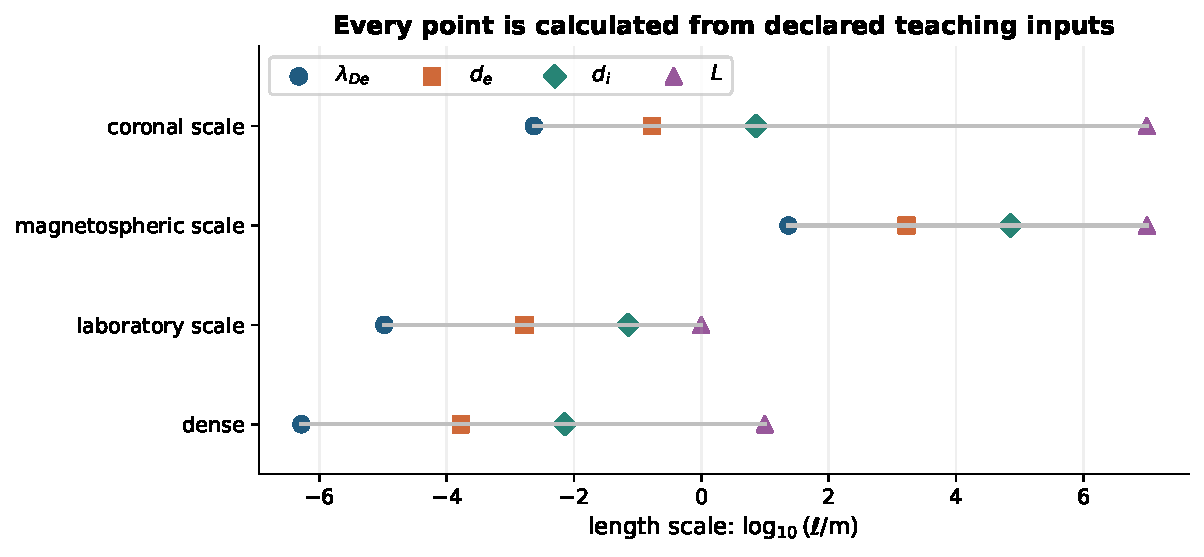
\includegraphics[width=.98\textwidth]{figures/03_scales.pdf}
\caption{四组教学输入对应的长度。横轴是米数的十进对数；间隔1代表长度相差10倍。$d_i/d_e$由质量比固定，而$L/d_i$与$\lambda_{De}/d_e$依参数改变。}\label{hall:figscales}\end{figure}

\subsection{例一：把实验室量级的每一步真的代进去}
取$n=10^{19}\,\mathrm{m^{-3}}$、$B=0.05\,\mathrm T$、$T_i=T_e=20\,\mathrm{eV}$、$L=1\,\mathrm m$。先算质量密度
\begin{equation}
\rho\simeq nm_i=1.67262\times10^{-8}\,\mathrm{kg/m^3}.
\end{equation}
因此
\begin{align}
V_A&=\frac{0.05}{\sqrt{(1.25664\times10^{-6})(1.67262\times10^{-8})}}
=3.4488\times10^5\,\mathrm{m/s},\\
\Omega_i&=\frac{(1.60218\times10^{-19})(0.05)}{1.67262\times10^{-27}}
=4.7894\times10^6\,\mathrm{s^{-1}},\\
d_i&=V_A/\Omega_i=0.07201\,\mathrm m,\\
d_e&=0.07201/\sqrt{1836.15}=1.6805\times10^{-3}\,\mathrm m,\\
\lambda_{De}&=\sqrt{\frac{(8.85419\times10^{-12})(3.20435\times10^{-18})}
{(10^{19})(1.60218\times10^{-19})^2}}
=1.0513\times10^{-5}\,\mathrm m.
\end{align}
电子压强$p_e=n\Theta_e=32.0435\,\mathrm{Pa}$，磁压$B^2/(2\mu_0)=994.72\,\mathrm{Pa}$，故$\beta_e=0.03221$。离子热速度$6.190\times10^4\,\mathrm{m/s}$，所以$\rho_i=0.01292\,\mathrm m$；$\rho_s=0.009139\,\mathrm m$。本例$d_i$约7.2厘米，而$\rho_i$约1.3厘米，二者不可互换。

密度换算为$10^{13}\,\mathrm{cm^{-3}}$后，
\begin{align}
\nu_{ei}&\simeq2.91\times10^{-6}\frac{10^{13}\times10}{20^{3/2}}
\simeq3.25\times10^6\,\mathrm{s^{-1}},\\
\eta_D&=\frac{(9.1094\times10^{-31})(3.2494\times10^6)}{(10^{19})(1.60218\times10^{-19})^2}
=1.1531\times10^{-5}\,\Omega\,\mathrm m,\\
D_\eta&=9.176\,\mathrm{m^2/s},\qquad
\lambda_{\rm mfp,e}=\frac{2.6524\times10^6}{3.2494\times10^6}=0.8163\,\mathrm m.
\end{align}
结果告诉我们：虽然有碰撞，电子沿温度变化长度的局地输运近似仍可能不成立；若沿场长度只有厘米，平均自由程明显更长。不能用“$\nu_{ei}$看起来很大”替代无量纲比较。

\subsection{例二：同一组参数，不同层厚得到不同模型}
取参考场$E_A=V_AB=1.7244\times10^4\,\mathrm{V/m}$，并暂取$\ell_B=\ell_p=\ell$。这是比较特征幅度，不是在X点把$U\times B$当作实际非零项。下表全部来自刚才的输入：
\begin{longtable}{P{29mm}rrrr}
\toprule 层厚$\ell$ & $1\,\mathrm m$ & $0.10\,\mathrm m$ & $0.010\,\mathrm m$ & $d_e=1.68\,\mathrm{mm}$\\\midrule
$E_H/E_A$ &0.0720&0.720&7.20&42.85\\
$E_p/E_A$ &0.00116&0.0116&0.116&0.690\\
$E_\eta/E_A$ &$2.66\times10^{-5}$&$2.66\times10^{-4}$&$2.66\times10^{-3}$&0.0158\\
$E_{m_e}/E_H$ &$2.82\times10^{-6}$&$2.82\times10^{-4}$&0.0282&1.00\\\bottomrule
\end{longtable}
最后一行分母是$E_H$，前三行分母是$E_A$，不能把四行直接相加。若要得到惯性相对$E_A$，应乘上第一行，例如$\ell=1$厘米时为$0.0282\times7.20=0.203$。到了$d_e$，忽略电子惯性的排序已经失败，不能继续用质量小作为理由。

在$\ell=0.1$米处，具体电场幅度为
\begin{align}
E_H&\sim0.720E_A=1.24\times10^4\,\mathrm{V/m},\\
E_p&\sim\Theta_e/(e\ell)=20/0.1=200\,\mathrm{V/m},\\
E_\eta&\sim\eta_D B/(\mu_0\ell)=4.59\,\mathrm{V/m}.
\end{align}
若该区域离子入流仅$0.1V_A$，对应的对流电场是$1.724\times10^3\,\mathrm{V/m}$，Hall幅度比值又大10倍。但真正要判断$E_z$时，必须用$(J_xB_y-J_yB_x)/(en)$，不能把$|J||B|/(en)$无条件塞给$z$分量。
\begin{figure}[htbp]\centering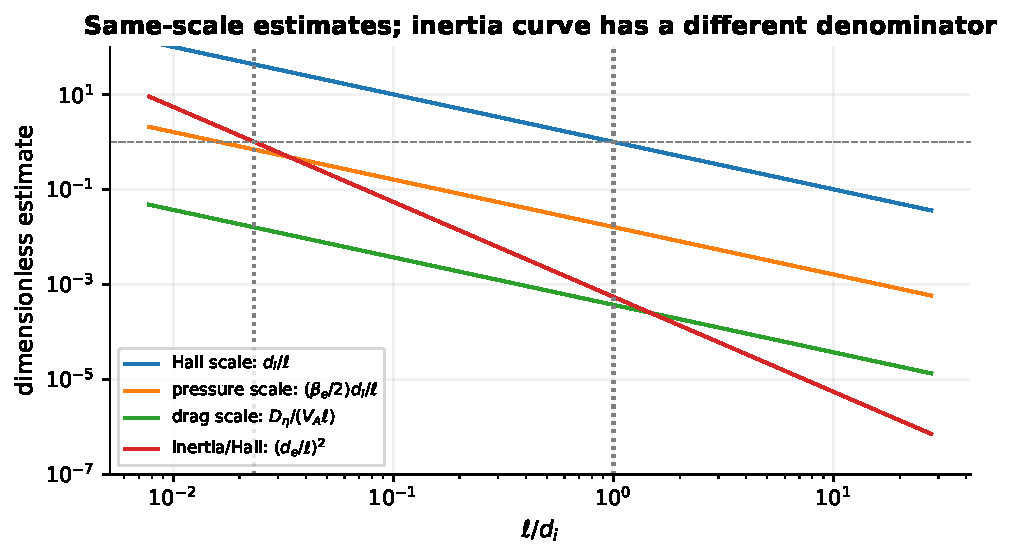
\includegraphics[width=.98\textwidth]{figures/04_ordering.pdf}
\caption{实验室教学参数下的同尺度估计。惯性曲线特意标明分母为Hall量级；其他三条除以$V_AB$。这些曲线表示排序如何随层厚改变，不是任何一次模拟的实测欧姆定律分解。}\label{hall:figordering}\end{figure}

\subsection{例三：为什么准中性成立而电子惯性仍要保留}
仍取实验室例，但$\ell=d_e=1.6805$毫米。假定$e\phi\sim\Theta_e$，电荷差相对密度为
\begin{equation}
\left(\frac{1.0513\times10^{-5}}{1.6805\times10^{-3}}\right)^2
=3.91\times10^{-5}.
\end{equation}
它很小，而$(d_e/\ell)^2=1$。因此\emph{准中性并不排除电子惯性}。若用Alfvén速度估计位移电流，其比值$(V_A/c)^2=1.32\times10^{-6}$。但电子流若达到电子Alfvén速度$V_{Ae}=V_A\sqrt{m_i/m_e}=1.478\times10^7\,\mathrm{m/s}$，相应估计上升至$2.43\times10^{-3}$；仍小，却不是前一个数。还应检查实际时间频率相对$\omega_{pe}$。

\subsection{例四：磁层不是把实验室的厘米改写成千米}
取$n=10^7\,\mathrm{m^{-3}}=10\,\mathrm{cm^{-3}}$、$B=20$ nT、$T_e=100$ eV、$T_i=1000$ eV。得到$V_A=138$ km/s、$d_i=72.0$ km、$d_e=1.68$ km、$\lambda_{De}=23.5$ m。离子$\beta_i=10.1$，所以
\begin{equation}
\rho_i=d_i\sqrt{\beta_i}=72.0\times\sqrt{10.1}\simeq228\,\mathrm{km}.
\end{equation}
如果层厚100 km，$d_i/\ell=0.720$，但$\rho_i/\ell=2.28$；Hall与离子有限轨道宽度都不能忽视。电子惯性/Hall约为$(1.68/100)^2=2.82\times10^{-4}$，暂小；电子压强量级/Hall约为$\beta_e/2=0.503$，已经不小。

$\nu_{ei}=5.81\times10^{-7}\,\mathrm{s^{-1}}$、$L/V_A=72.5$秒，所以$\nu_{ei}\tau_A=4.21\times10^{-5}$。沿系统通过的时间内，库仑碰撞极少；由此计算出的经典电阻只能作为很小的参照，不能把它当成已经证明能负责破冻结的机制。

\subsection{例五：强导场下必须分清哪个磁场进入哪个尺度}
在实验室例中保留反向分量$B_r=0.05$ T，另加$B_g=0.50$ T。重联可释放的反向场能量和对应$V_{Ar}$仍用$B_r$；回旋运动感受到的总场约$0.5025$ T。因此回旋半径约缩小为原来的$0.05/0.5025=0.0995$倍：$\rho_i\simeq1.286$毫米，$\rho_s\simeq0.909$毫米；$d_i=72.0$毫米完全不变，因为惯性长度不含$B$。

若需要判断强导场下的离子声/有限回旋效应，$\rho_s$可能比$d_i$更相关；若需要估计由反向场梯度形成的电流，分子仍是$B_r$。这一步明确后，才谈“Hall尺度由哪一个长度控制”；不能只替换一个符号便声称所有反平行结论都成立。

\section{例六：改变电子质量会具体改变什么}
很多计算把$m_i/m_e$从1836改成100或25以降低成本。在$n,B,m_i$固定时，$d_i,V_A,\Omega_i$不变，而$d_e/d_i$依次为0.02334、0.10、0.20。若每个$d_e$用8格，$100d_i$宽的方向所需格数为
\begin{align}
N_{1836}&=100d_i/(d_e/8)=34280,\\
N_{100}&=8000,\qquad N_{25}=4000.
\end{align}
二维格数约按一维格数平方增长，三维更昂贵。这解释了缩质量比的动力。但电子热速度、惯性响应、$\Omega_e$以及两个层的分离都随之改变；它不只是把计算钟变快。应至少比较一组质量比序列，并固定清楚物理或无量纲输入，不能把缩质量比的一张温图当成真实质量比结论。
